\chapter{Our contributions}
\label{chap3}

\section{Triangulation adaptive to the local curvature}
\label{sub3.1}

\section{Triangulation of ADE singularities}
\label{sub3.2}

\subsection*{Analysis of the geometry of ADE singularities}

ADE singularities are simple, isolated surface singularities, which can be
expressed by corresponding implicit equations.

We already know, that $A_{1--}$ singularity is locally represented as a cone.
In this section we will discuss geometric structure of other ADE surface singularities.

\begin{definition} TODO rewrite
    Let's define branch of ADE singularity as the part of surface,
    which is connected to the rest only by the singular point.
\end{definition}

\begin{comment}
\begin{definition}
    Let's define traingulation direction of ADE singularity $A$ with radius $r$ as 
    a direction $\overrightarrow{v}$ for which 
    $$F\bigg(A+t \overrightarrow{v} \cap S_{r}(A)\bigg) < 0,$$
    where $F$ is the implicit equation defining the singularity $A$
    and $t,r \in \R^+$.
\end{definition}
As we can see, there are infinitely many axes of each ADE singularity.
\end{comment}

For our needs, we will pick one triangulation vector for each branch of
each ADE singularity. This trinauglation vector is either in the direction
of rotation symmetry axis or an intersection of reflection symmetry planes
of the corresponding branch.

\begin{comment}
Moreover, when placed to the singular point, triangulation vector of a branch 
is in the same half-space as the corresponding branch.
\end{comment}

In the general case, triangulation vectors will serve
as an orientation of a singularity with respect to its normal form.

\subsubsection*{$A_n$ singularities}

As we can see from the equations 
$F(x,y,z)=x^{n+1}\pm y^2\pm z^2$, $A_{n-+}$
singularities are just rotated $A_{n+-}$ singularities and $A_{n++}$ singularities
are a single point if $n$ is odd and reflected $A_{n--}$ singularities if n is even. 
We will therefore only discuss geometry of $A_{n--}$ and $A_{n+-}$ singularities.

$A_{n--}$ singularities are topologically equivalent to a cone if $n$ is odd, therefore
they have two branches.
If $n$ is even, they are topologically equivalent to a half cone or a plane, therefore
they have a single branch.
As $n$ gets bigger, the tip of the cone gets sharper. As $A_{n--}$ singularities
are rotationally symmetrical, we will pick the direction of
axis of symmetry as triangulation vector. For a normal form, the triangulation vectors
are $(1, 0, 0)$ (and $(-1, 0, 0)$ if n is odd).
First four $A_{n--}$ singularities can be seen on image \ref{img:4}.

\begin{figure}
    \centerline{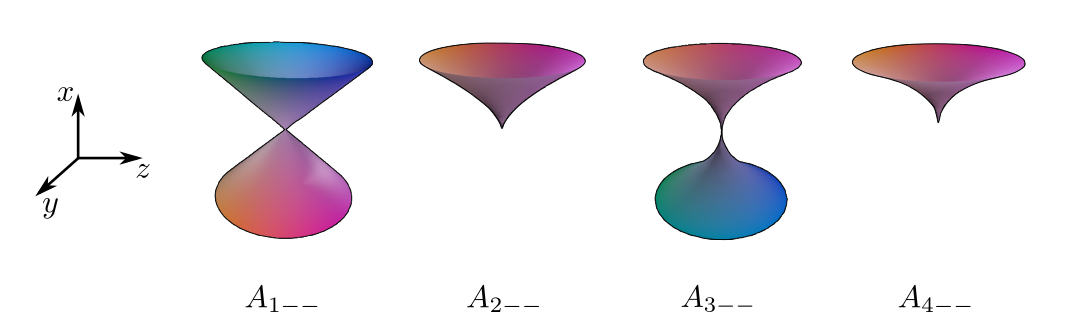
\includegraphics[width=1\textwidth]{images/img4}}
    \caption[$A_{n--}$ singularities]
    {$A_{n--}$ singularities. \cite{singsurf}}
    %id obrazku, pomocou ktoreho sa budeme na obrazok odvolavat
    \label{img:4}
\end{figure}


$A_{n+-}$ singularities are topologically equivalent to a cone if $n$ is odd, therefore
they have two branches.
In the contrary with the previous singularities, as $n$ gets bigger, the tip
of the cone gets less sharp and flatter. Branches of these singualrities have 
reflection symmetry planes $x=0$ and $y=0$, therefore we will pick the vectors
$(0, 0, 1)$ and $(0, 0, -1)$ as the triangulation vectors.

If $n$ is even, $A_{n+-}$ singualrities are topologically equivalent to a plane
with shape similar to hyperbolic paraboloid, therefore they have a single branch.
First four $A_{n+-}$ singularities can be seen on image \ref{img:5}.
For this case, we will pick the vector $(1, 0, 0)$ as a triangulation vector as
these singularities have reflection symmetry planes $y=0$ and $z=0$.

\begin{figure}
    \centerline{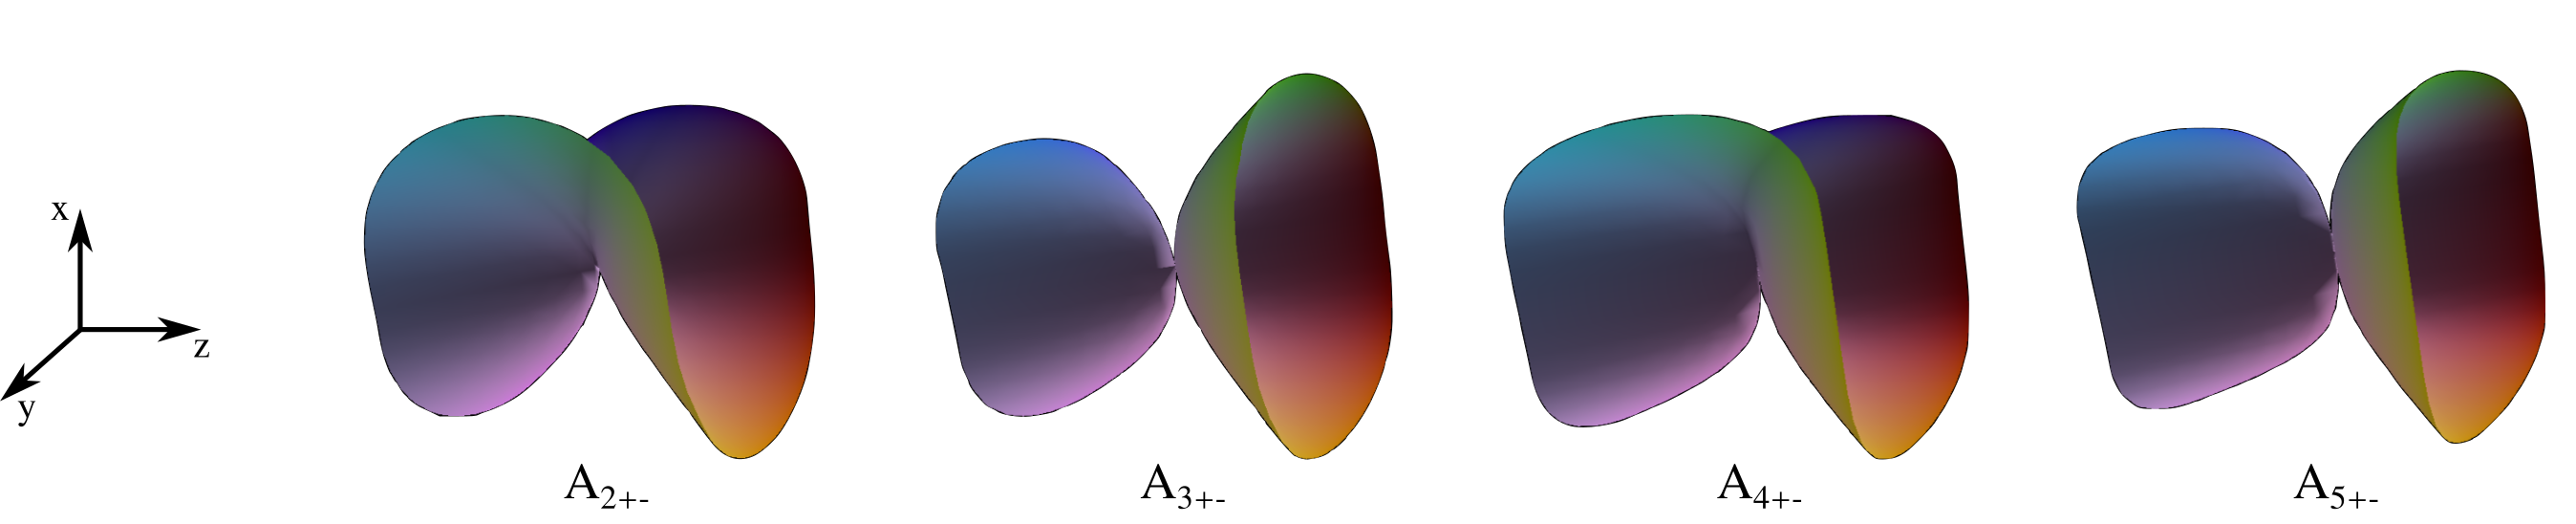
\includegraphics[width=1\textwidth]{images/img5}}
    \caption[$A_{n+-}$ singularities]
    {$A_{n+-}$ singularities. \cite{singsurf}}
    %id obrazku, pomocou ktoreho sa budeme na obrazok odvolavat
    \label{img:5}
\end{figure}

\subsubsection*{$D_n$ singularities}

Given by equations $F(x,y,z)=yx^2\pm y^{n-1}\pm z^2$, we will consider 8 categories.
For given sign combination and parity of n, the singularities are topologically
equivalent, with sharper(or flatter) features around the singualrities for increasing
value of $n$ similar to $A_n$ singualrities.

We can therefore say that $D_n$ singularities can be classified into 8 categories
represented by the following singularities:
\begin{itemize}
    \item $D_{4++}$ \hspace{5mm} $yx^2 + y^3 + z^2$
    \item $D_{5++}$ \hspace{5mm} $yx^2 + y^4 + z^2$
    \item $D_{4+-}$ \hspace{5mm} $yx^2 + y^3 - z^2$
    \item $D_{5+-}$ \hspace{5mm} $yx^2 + y^4 - z^2$
    \item $D_{4-+}$ \hspace{5mm} $yx^2 - y^3 + z^2$
    \item $D_{5-+}$ \hspace{5mm} $yx^2 - y^4 + z^2$
    \item $D_{4--}$ \hspace{5mm} $yx^2 - y^3 - z^2$
    \item $D_{5--}$ \hspace{5mm} $yx^2 - y^4 - z^2$.
\end{itemize}

Now we will look at some equivalences between these 8 categories.
$D_{4++}$ singularity is reflected $D_{4+-}$ singularity.
$D_{5++}$ singularity is reflected $D_{5--}$ singularity.
$D_{5-+}$ singularity is reflected $D_{5+-}$ singularity.
$D_{4-+}$ singularity is reflected $D_{4--}$ singularity.

We will therefore only analyze geometry of $D_{n+-}$ singualrities and
$D_{n--}$ singularities.

$D_{n+-}$ singularities are topologically equivalent to a plane when $n$ is
even and to a cone when $n$ is odd. Again, as $n$ gets bigger, the features
around singularities get sharper. Symmetry planes of these singularities
are $x=0$ and $z=0$, therefore we pick $(0, 1, 0)$ (and $(0, -1, 0)$ when $n$ is odd)
as trinauglation vectors. First four $D_{n+-}$ singularities can be seen on
image \ref{img:7}.

\begin{figure}
    \centerline{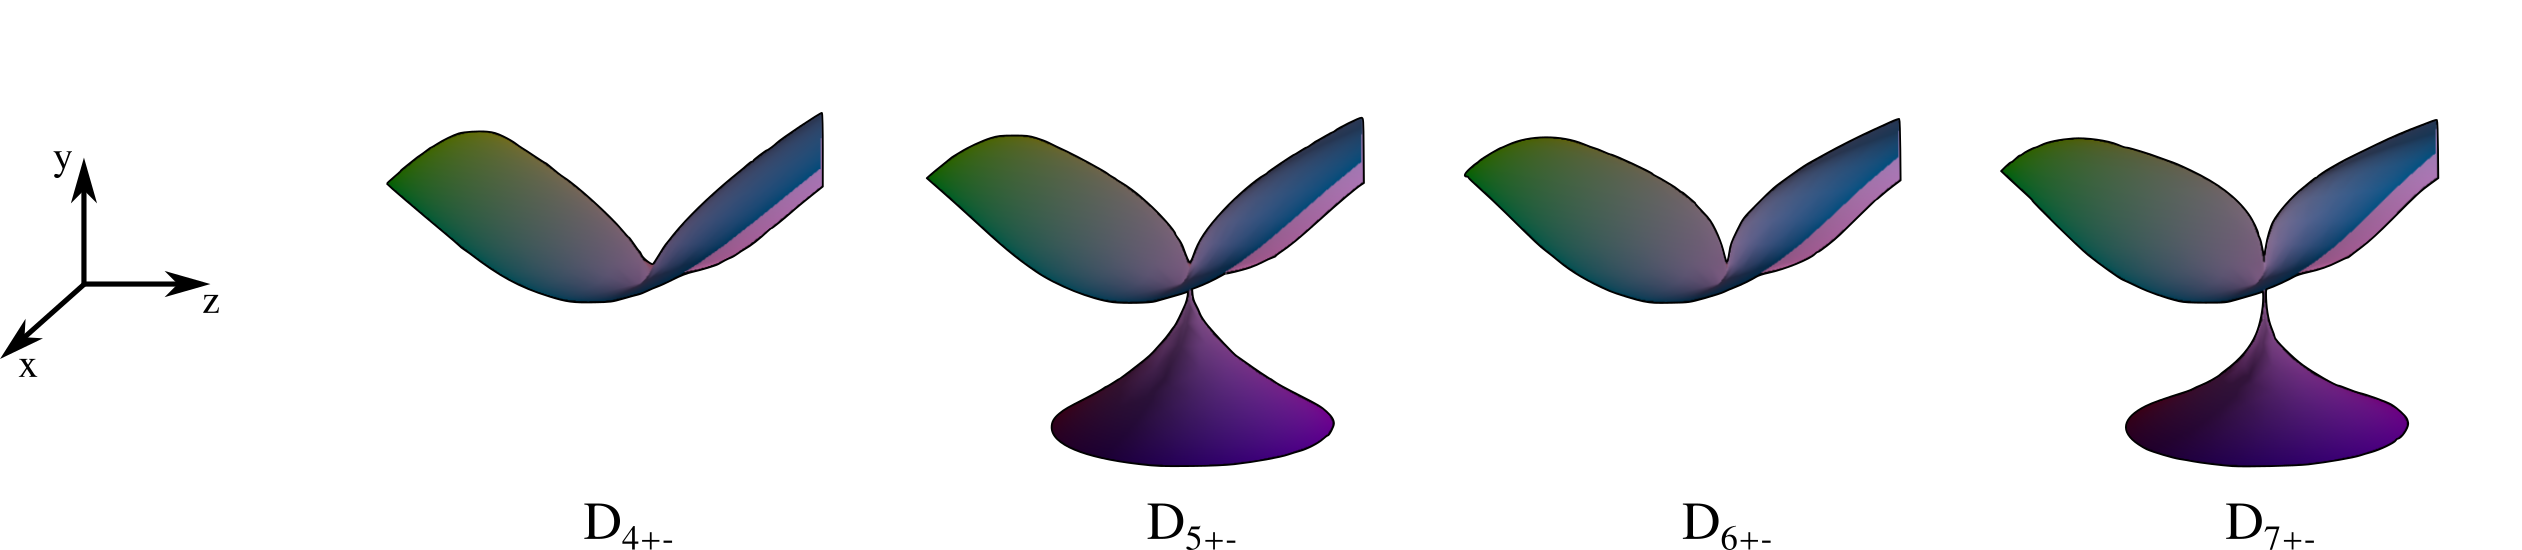
\includegraphics[width=1\textwidth]{images/img7}}
    \caption[$D_{n+-}$ singularities]
    {$D_{n+-}$ singularities. \cite{singsurf}}
    %id obrazku, pomocou ktoreho sa budeme na obrazok odvolavat
    \label{img:7}
\end{figure}


$D_{n--}$ singularities are topologically equivalent to a cone when $n$ is
odd and to a 3 halfcones connected in the singular point when $n$ is even.
First four $D_{n--}$ singularities can be seen on image \ref{img:8}.

\begin{figure}
    \centerline{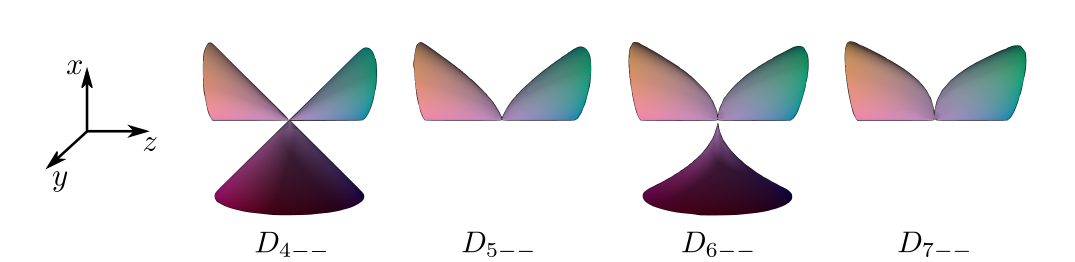
\includegraphics[width=1\textwidth]{images/img8}}
    \caption[$D_{n--}$ singularities]
    {$D_{n--}$ singularities. \cite{singsurf}}
    %id obrazku, pomocou ktoreho sa budeme na obrazok odvolavat
    \label{img:8}
\end{figure}

Symmetry plane for all branches of these singularities is $z=0$.
the intersection of the surface and plane $z=0$ is displayed on image \ref{img:6}.

\begin{figure}
    \centerline{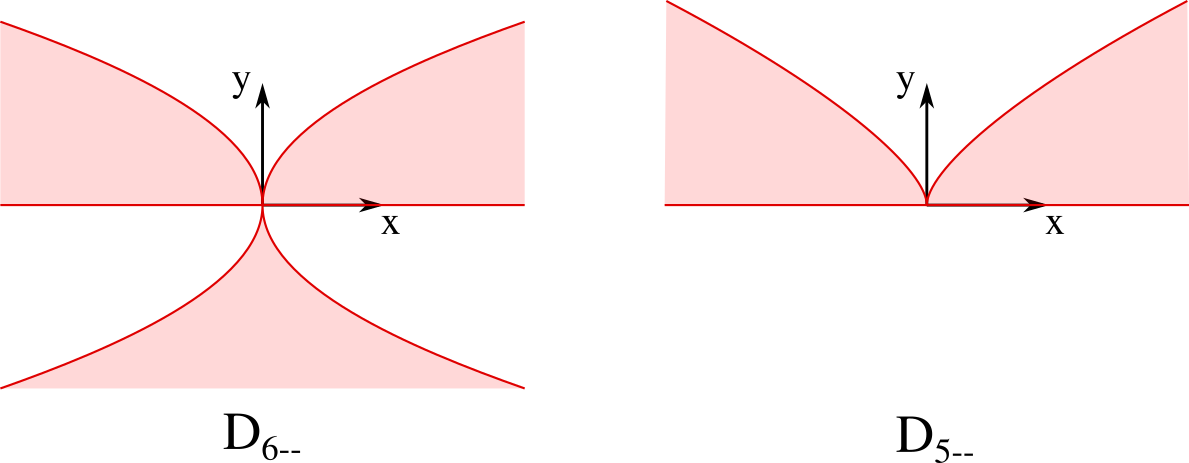
\includegraphics[width=0.7\textwidth]{images/img6}}
    \caption[Intersection of $D_{n--}$ singularities with plane $z=0$.]
    {Intersection of $D_{n--}$ singularities with plane $z=0$.}
    %id obrazku, pomocou ktoreho sa budeme na obrazok odvolavat
    \label{img:6}
\end{figure}

For $D_{n--}$ singularity, the intersections of the two branches where
$y \geq 0$ are bounded by curves $y=0$ and $x^2=y^{n-2}$. For given $r$,
we will pick the triangulation vectors as $(r, \frac{1}{2}r^{\frac{2}{n-2}}, 0)$
and $(-r, \frac{1}{2}r^{\frac{2}{n-2}}, 0)$. The resulting vectors are
displayed on image \ref{img:9} by blue arrow.

\begin{figure}
    \centerline{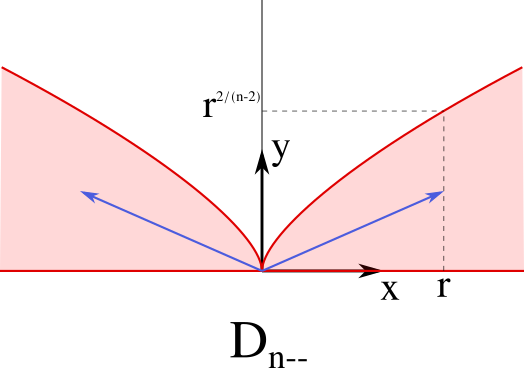
\includegraphics[width=0.35\textwidth]{images/img9}}
    \caption[Triangulation vectors for two branches of $D_{n--}$ singularities.]
    {Triangulation vectors for two branches of $D_{n--}$ singularities.}
    %id obrazku, pomocou ktoreho sa budeme na obrazok odvolavat
    \label{img:9}
\end{figure}

The third branch where $y\leq0$ has has another plane of symmetry $x=0$,
therefore triangulation vector for this branch is chosen as $(0, -1, 0)$.

\subsubsection*{$E_6, E_7$ and $E_8$ singularities}

Given by equations $F(x,y,z)=x^3\pm y^4\pm z^2$, $F(x,y,z)=x^3\pm xy^3\pm z^2$
and $F(x,y,z)=x^3\pm y^5\pm z^2$, we can see the following equivalences:
$E_{6++}$ singularity is reflected $E_{6--}$ singularity.
$E_{6+-}$ singularity is reflected $E_{6-+}$ singularity.
$E_{7+-}, E_{7-+}$ and $E_{7--}$ are all reflected $E_{7++}$ singularity.
$E_{8+-}, E_{8-+}$ and $E_{8--}$ are all reflected $E_{8++}$ singularity.

We will only analyze geometry of $E_{6++}$, $E_{6+-}$, $E_{7++}$ and $E_{8++}$
singularities.

Both $E_{6++}$ and $E_{6+-}$ are topologically equivalent to a plane, thus
they each have only one branch. The planes of symmetry of both of these 
branches are $y=0$ and $z=0$, therefore we pick $(-1, 0, 0)$ as the
triangulation vector.

$E_{7++}$ singularity is topologically equival to a cone, therefore it has
two branches. The plane of symmetry of this singularity is $z=0$.

$E_{8++}$ singularity is also topologically equivalent to a plane, therefore
it has only one branch. This branch has only one plane of symmetry $z=0$.

We will again look at the intersection of the surfaces with the plane of 
symmetry, this is displayed on image \ref{img:10}.

\begin{figure}
    \centerline{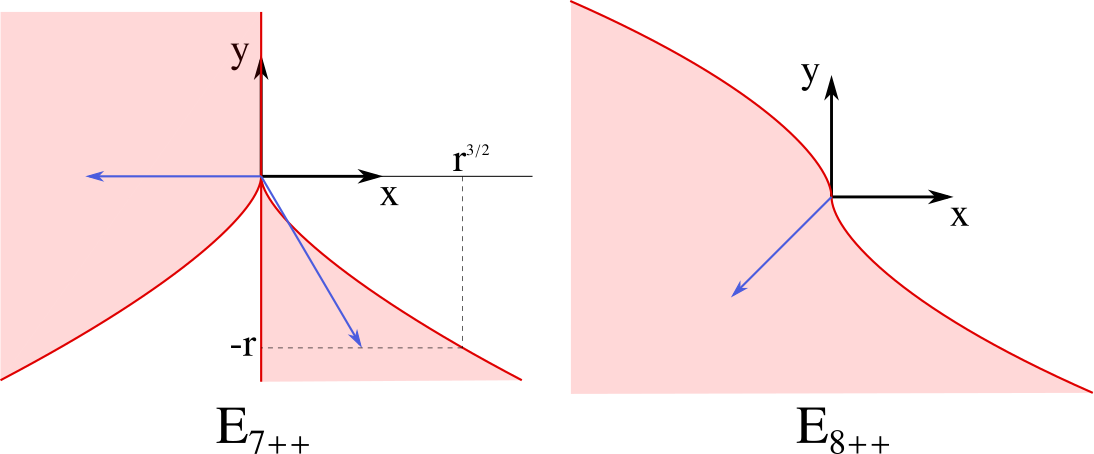
\includegraphics[width=0.6\textwidth]{images/img10}}
    \caption[Intersection of $E_{7++}$ and $E_{8++}$ singularities with 
    plane $z=0$.]
    {Intersection of $E_{7++}$ and $E_{8++}$ singularities with 
    plane $z=0$.}
    %id obrazku, pomocou ktoreho sa budeme na obrazok odvolavat
    \label{img:10}
\end{figure}

For $E_{7++}$ singularity, we will pick $(-1, 0, 0)$ and 
$(\frac{1}{2}r^{\frac{3}{2}}, -r, 0)$ as triangulation vectors.
For $E_{8++}$ singularity, we will pick $(-1, -1, 0)$ as a triangulation vector.
These vectors are displayed on the image \ref{img:10} as blue arrows.

\subsection*{Analytical calculation of local triangulation of some ADE singularities}
For given edge size $e$, we want to calculate the local triangulation of ADE
singularities, such that edges on the border of the local triangulation
have length $e$.
\subsubsection*{$A_{n--}$ singualrities}
For $A_{n--}$ singularities, we create a disc of $6$ isosceles triangles
with vertex in the singular point. The bases of these triangles create regular
hexagon in the plane $P$ parallel to the plane $x=0$, as showed on the image
\ref{img:11}
\begin{figure}
    \centerline{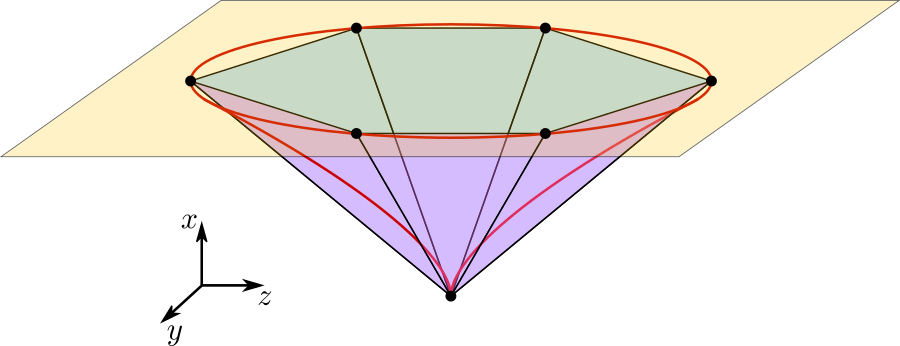
\includegraphics[width=0.6\textwidth]{images/img11}}
    \caption[Triangulation of $A_{n--}$ singularity.]
    {Triangulation of $A_{n--}$ singularity.}
    %id obrazku, pomocou ktoreho sa budeme na obrazok odvolavat
    \label{img:11}
\end{figure}
Given by equation $x^{n+1}-y^2-z^2=0$, we will find the distance of the 
plane $P$ from the plane $x=0$ for the given length $e$ of the sides of
the hexagon.

Let $e$ be the length of the side of the hexagon, then the circumscribed
circle has radius $e$. This circle is identical with the intersection of
the surface and the plane $x=h$. The equation of the intersecting circle
is $y^2+z^2=h^{n+1}$ therefore, the radius can be also expressed as 
$r=h^{\frac{n+1}{2}}$, which emerges $h=e^{\frac{2}{n+1}}$. Knowing the
distance of the plane, one can easily calculate the length of the arms of
the triangles using Pythagorean theorem: 
$$a^2=h^2+e^2 \implies a = \sqrt{e^{\frac{4}{n+1}} + e^2}$$

\subsubsection*{$D_n$ singualrities}
\subsubsection*{$E_6, E_7$ and $E_8$ singualrities}

\subsection*{Numerical calculation of local triangulation of ADE singularities}


\section{Triangulation of non-isolated singularities of translation surfaces}
\label{sub3.3}
